\chapter{Chain Complexes}

%\pagenumbering{arabic}

\section{Introduction}

A\index{chain complex} {\em chain complex}\footnote{{\bf P.J. Giblin} in
{\em Graph, Surface and Homology}, Chapman and Hall Math. series, 1981.}
($C_p, d_p$) is a collection of free $\Z$--modules ($C_p$), one for each
$p \in \Z$, together with a homomorphism $d_p : C_p \rightarrow C_{p-1}$, such
that, for all $p$, $d_{p-1} \circ d_p = 0$.
\par
{\bf In the Kenzo program}, a  {\em  morphism}\index{morphisms! in {\tt Kenzo}} $f=(f_p)$, of degree $k$,
from a chain complex ($C_p, d_p$) to another ($C'_p, d'_p$) is a
collection of homomorphisms
$$f_p : C_p \rightarrow C'_{p+k}.$$
This is expressed by the following  diagram, generally {\bf not assumed commutative}.

$$\diagram{
\cdots & \leftarrow & C_{p-1} & \buildrel {d_p} \over \longleftarrow
                     & C_p     & \buildrel {d_{p+1}} \over \longleftarrow
                     & C_{p+1}
       & \leftarrow & \cdots \cr
       &             & \vfl {\displaystyle {f_{p-1}}}{}
       &             & \vfl {\displaystyle {f_p}}{}
       &             & \vfl {\displaystyle {f_{p+1}}}{} \cr
\cdots & \leftarrow & C'_{p+k-1} & \buildrel {d'_{p+k}} \over \longleftarrow
                     & C'_{p+k}     & \buildrel {d'_{p+k+1}} \over \longleftarrow
                     & C'_{p+k+1}
       & \leftarrow & \cdots \cr }
$$

\newpage
Three types of   morphisms are most generally considered.
\begin{enumerate}
\item $k=0$. If the commutativity relation $d'_p\circ f_p=f_{p-1}\circ d_p$ holds for every $p$, then the morphism
$f$ is an ordinary chain complex morphism or {\em chain map}\index{chain map}.
\item $k=-1$. If $(C_p,d_p)=(C'_p,d'_p)$ and $f_p=d_p$, then $f$ is the
{\em differential}\index{chain complex!differential} of the chain complex
$(C_p,d_p)$ and, in fact, this differential is implemented in the {\tt Kenzo} program as a morphism of degree $-1$.
\item $k=+1$. In this case, $f$ is usually a {\em homotopy operator}\index{homotopy operator}, that is, some relation
$$d'_{p+1}\circ f_p+f_{p-1}\circ d_p=g_p-g'_p$$
is satisfied for two (ordinary) chain complex morphisms $g$ and $g'$.
\end{enumerate}
For technical reasons, these three types of morphisms have been implemented in the {\tt Kenzo} program
in a unique type.

\section {Generators, terms and combinations}

To become familiar to the lisp functions implementing the chain complexes, the best is to begin
by an example of chain complex. The {\em simplicial complexes}\index{simplicial complexes} are good candidates
for this purpose and we shall take as typical example the following simplicial
complex.
%
\vskip 0.50cm
\centerline{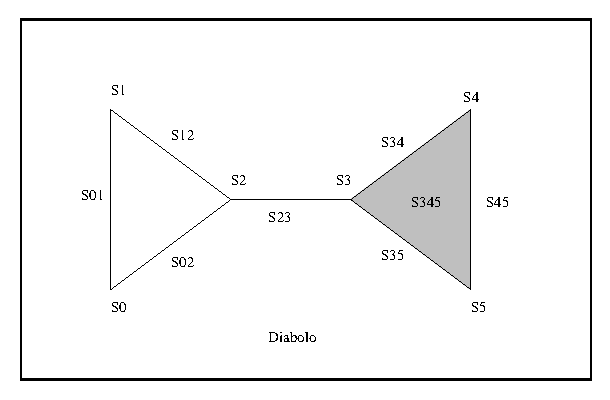
\includegraphics{diabolo.eps}}
%\centerline{\psfig{figure=diabolo.eps}}
\vskip 0.50cm
%
In this simplicial complex, called here {\em diabolo}, there are $3$ associated chain groups.
\begin{itemize}
\item $C_0$, the free $\Z$--module on the set of vertices $\{s_0,s_1,s_2,s_3,s_4,s_5 \}$.
\item $C_1$, the free $\Z$--module on the set of  edges
   $\{ s_{01}, s_{02}, s_{12}, s_{23}, s_{34}, s_{35}, s_{45} \}$.
\item $C_2$, the free $\Z$--module on the set of  triangles (here a singleton)
   $\{ s_{345} \}$.
\end{itemize}
The elements of either of those groups $C_p$ are linear integer combinations  of the
corresponding basis\index{chain complex!basis} (set of $\sigma_i$'s), i.e. elements of the form:
$$ \sum {\lambda_i \sigma_i}, \quad \lambda_i \in \Z. $$
An element $\sigma_i$ of any basis is also called {\em generator}\index{generator} and in our specific case
this generator will be represented by a  lisp symbol. For instance,
$s_{45}$ will be translated in {\tt s45}. But, the user must know from now, that in the realistic
usage of the software, generators may be of any type.
A product such as $\lambda_i \sigma_i$ is called
a {\em term}\index{term} and a sum of terms, a {\em combination}\index{combination}.

\subsection {Representation of a combination}

A combination\index{combination!representation} is represented internally in the system by a  list
having the general following form:
\begin{center}
{\tt (:cmbn {\em degree} $(\lambda_1.\sigma_1)$ ... $(\lambda_k.\sigma_k)$)}
\end{center}
and containing
\begin{enumerate}
\item The degree of the combination  corresponding to the index $p \in \Z$  of the group
$C_p$ to which this combination belongs.
\item The  list of the internal representation of the terms, namely the list of pairs $(\lambda_i.\sigma_i)$.
\end{enumerate}
This choice of representation implies that only homogeneous combinations
will be considered. A type {\tt CMBN} and
a printing method have been associated to this internal representation. The external
form of a combination is shown in the  examples.

\subsection {Ordering the generators}

In order\index{generator!ordering} to speed up the execution of algorithms involving combinations,
the list of pairs $(\lambda_i.\sigma_i)$ is ordered by an adequate ordering function (ex: the  lexicographical ordering
on the symbols). For programming convenience, an enumerated type {\tt CMPR} has been defined:
{\footnotesize\begin{verbatim}
(deftype cmpr() '(member :less :equal :greater))
\end{verbatim}}
A number of macros, functions and methods have been defined
on usual sets (symbols, numbers, lists, ...) taking their value in the set
{\tt [:less, :equal, :greater]}. Of course, the user may define its own function for a particular case.
There exists functions to compare various couples of usual items:
\vskip 0.45cm
{\parindent=0mm
{\leftskip=5mm
{\tt f-cmpr} {\em n1 n2}\hfill {\em [Function]} \par}
{\leftskip=12mm
Return {\tt :less}, {\tt :equal}, {\tt :greater}, according to the result of
the canonical comparison of both integers {\em n1} and {\em n2}. \par}
{\leftskip=5mm
{\tt s-cmpr} {\em symbol1 symbol2} \hfill {\em [Function]}\par}
{\leftskip=12mm
Return  {\tt :less}, {\tt :equal}, {\tt :greater}, according to the result of
the lisp comparison functions on the strings {\tt (symbol-name {\em symbol1})}
and {\tt (symbol-name {\em symbol2})} \par}
{\leftskip=5mm
{\tt l-cmpr} {\em list1 list2}\hfill {\em [Function]} \par}
{\leftskip=12mm
Return  {\tt :less}, {\tt :equal}, {\tt :greater}, according to the
lexicographical ordering of the two lists  {\em list1}
and {\em list2} representing legal generators in this implementation. \par}
}

\subsection* {Examples}

{\footnotesize\begin{verbatim}
(f-cmpr 123 789)  ==>

:LESS

(s-cmpr 'circulation 'circular)  ==>

:GREATER

(s-cmpr 'qwerty 'qwerty)  ==>

:EQUAL

(l-cmpr '(1 a b) '(1 a))  ==>

:GREATER
\end{verbatim}}
\newpage

\subsection {Functions handling  combinations}

The software provides a set of functions, methods or macros to create or modify
combinations\index{combination!handling}.
\vskip 0.45cm
{\parindent=0mm
{\leftskip=5mm
{\tt term-cmbn} {\em dgr cf gnr} \hfill {\em [Macro]}\par}
{\leftskip=15mm
Construct the combination of degree {\em dgr} with unique term $cf * gnr$ \par}
{\leftskip=5mm
{\tt cmbn} {\em dgr cf1 gnr1 cf2 gnr2 ... cfn gnrn}\hfill {\em [Function]} \par}
{\leftskip=15mm
Construct a combination of degree {\em dgr}, sum of the terms $cf_i *  gnr_i$. The sequence of pairs
$\lbrace cf_i\  gnr_i \rbrace$ has an undefinite length and  may be void. In this case,  the combination
is a null combination of degree {\em dgr}.  \par}
{\leftskip=5mm
{\tt cmbn-p} {\em object} \hfill {\em [Function]}\par}
{\leftskip=15mm
Test is {\em object} is a legal combination. \par}
{\leftskip=5mm
{\tt cmbn-degr} {\em cmbn}   \hfill {\em [Macro]} \par}
{\leftskip=15mm
Get the degree (an integer) of the combination {\em cmbn}. \par}
{\leftskip=5mm
{\tt cmbn-list} {\em cmbn}   \hfill {\em [Macro]} \par}
{\leftskip=15mm
Get the list of the terms  of the combination {\em cmbn}. Beware: a term is not a {\tt Kenzo} object.
One may select the coefficient (an integer) or the generator -- a {\tt Kenzo} object --
respectively by the macros {\tt cffc} and {\tt gnrt}. \par}
{\leftskip=5mm
{\tt zero-cmbn} {\em dgr}   \hfill {\em [Function]} \par}
{\leftskip=15mm
Create an instance of a null combination in the degree {\em dgr}. \par}
{\leftskip=5mm
{\tt zero-pure-dffr} {\em cmbn} \hfill {\em [Function]} \par}
{\leftskip=15mm
Create  a null combination of degree $degr(cmbn) - 1$. \par}
{\leftskip=5mm
{\tt cmbn-zero-p} {\em cmbn} \hfill {\em [Macro]}\par}
{\leftskip=15mm
Test if {\em cmbn} is a null combination in any degree. \par}
{\leftskip=5mm
{\tt cmbn-non-zero-p} {\em cmbn} \hfill {\em [Macro]} \par}
{\leftskip=15mm
Test if {\em cmbn} is a non-null combination in any degree. \par}
{\leftskip=5mm
{\tt cmbn-opps} {\em cmbn} \hfill {\em [Function]} \par}
{\leftskip=15mm
Create a  combination opposite to {\em cmbn}. \par}
{\leftskip=5mm
{\tt n-cmbn} {\em n cmbn} \hfill {\em [Function]} \par}
{\leftskip=15mm
Create a  combination multiple of  {\em cmbn} by the factor $n$. \par}
{\leftskip=5mm
{\tt 2cmbn-add} {\em cmpr cmbn1 cmbn2} \hfill {\em [Function]} \par}
{\leftskip=15mm
Create a combination, sum of both combinations {\em cmbn1} and {\em cmbn2}. The first
argument, {\em cmpr}, must be a function or macro relevant to compare the generators of the
involved combinations, in order to return an ordered combination. \par}
}
\newpage
{\parindent=0mm
{\leftskip=5mm
{\tt ncmbn-add} {\em cmpr cmbn1 cmbn2 ... cmbnk} \hfill {\em [Function]} \par}
{\leftskip=15mm
Create a combination, sum of the indefinite number of combinations $cmbn_i$. As to the first
argument, {\em cmpr}, see the function {\tt 2cmbn-add}. \par}
{\leftskip=5mm
{\tt 2n-2cmbn} {\em cmpr n1 cmbn1 n2 cmbn2} \hfill {\em [Function]} \par}
{\leftskip=15mm
Build the combination $n1 * cmbn1 + n2 * cmbn2$. Both integers $n1$ and $n2$ must be
non null. As to the first argument, {\em cmpr}, see the function {\tt 2cmbn-add}. \par}
{\leftskip=5mm
{\tt 2cmbn-sbtr} {\em cmpr cmbn1 cmbn2} \hfill {\em [Function]} \par}
{\leftskip=15mm
Create a combination, difference of {\em cmbn1} and {\em cmbn2}.
As to the first argument, {\em cmpr}, see the function {\tt 2cmbn-add}. \par}
}
\subsection* {Examples}

{\footnotesize\begin{verbatim}
(setf comb1 (cmbn 1 1 'u 2 'v 3 'w 4 'z))  ==>
-----------------------------------------------------------------------{CMB 1}
<1 * U>
<2 * V>
<3 * W>
<4 * Z>
------------------------------------------------------------------------------

(cmbn-non-zero-p comb1)  ==>

T

(cmbn-list comb1)  ==>

((1 . U) (2 . V) (3 . W) (4 . Z))

(setf term3 (third *))  ==>  ;; not a Kenzo object!

(3 . W)

(cffc term3)  ==>

3

(gnrt term3)  ==>

W
\end{verbatim}}
\newpage
{\footnotesize\begin{verbatim}
(setf mcomb1 (cmbn-opps comb1))   ==>

-----------------------------------------------------------------------{CMB 1}
<-1 * U>
<-2 * V>
<-3 * W>
<-4 * Z>
------------------------------------------------------------------------------

(setf comb2 (n-cmbn 10 comb1))  ==>

-----------------------------------------------------------------------{CMB 1}
<10 * U>
<20 * V>
<30 * W>
<40 * Z>
------------------------------------------------------------------------------

(setf cmb12 (2cmbn-add #'s-cmpr comb1 comb2))  ==>

----------------------------------------------------------------------{CMBN 1}
<11 * U>
<22 * V>
<33 * W>
<44 * Z>
------------------------------------------------------------------------------

(2cmbn-sbtr #'s-cmpr comb1 cmb12)  ==>

----------------------------------------------------------------------{CMBN 1}
<-10 * U>
<-20 * V>
<-30 * W>
<-40 * Z>
------------------------------------------------------------------------------

(ncmbn-add #'s-cmpr
           comb1 comb2 comb1 comb2 comb1 comb2 comb1 comb2  comb1 comb2)  ==>

----------------------------------------------------------------------{CMBN 1}
<55 * U>
<110 * V>
<165 * W>
<220 * Z>
------------------------------------------------------------------------------

\end{verbatim}}
\newpage

\section {Representation of a chain complex}

A chain complex\index{chain complex!representation} is implemented as an instance of a {\tt CLOS} class,
the class {\tt CHAIN-COMPLEX}\index{class!{\tt CHAIN-COMPLEX}}, whose definition is
{\footnotesize\begin{verbatim}
(DEFCLASS CHAIN-COMPLEX ()
    ((cmpr  :type cmprf :initarg :cmpr  :reader cmpr1)
     (basis :type basis :initarg :basis :reader basis1)
     ;; BaSe GeNerator
     (bsgn :type gnrt :initarg :bsgn :reader bsgn)
     ;; DiFFeRential
     (dffr :type morphism :initarg :dffr :reader dffr1)
     ;; GRound MoDule
     (grmd :type chain-complex :initarg :grmd :reader grmd)
     ;; EFfective HoMology
     (efhm :type homotopy-equivalence :initarg :efhm :reader efhm)
     ;; IDentification NuMber
     (idnm :type fixnum :initform (incf *idnm-counter*) :reader idnm)
     ;; ORiGiN
     (orgn :type list :initarg :orgn :reader orgn)))
\end{verbatim}}
This class has $8$ slots:
\begin{enumerate}
\item {\tt cmpr}, a comparison function or method for  generators with a range in the set
{\tt [:less, :equal, :greater]}.
\par
It is very important to note that the generators to be compared are assumed to be
of the {\em same degree}, i.e. they must belong to the same group $C_p$. As an exception with
the general policy of the software, this degree is not explicitly precised.
The implementor has chosen to avoid additional tests because in real problems the program spends
a lot of time comparing generators.
\item {\tt basis}, a lisp function giving the distinguished {\bf ordered} basis of the free $\Z$--modules\footnote{
Recall that in the software, only free chain complexes are considered.} ($C_p$).  When
some  components of the chain complex  are not finitely generated, we say that the chain complex
is {\em locally effective}. In this case the value of this slot must be the keyword
{\tt locally-effective}.
\item {\tt bsgn}, a lisp object of any type representing a distinguished generator in dimension $0$, the
base generator.
\item {\tt dffr}, the differential morphism, instance of the class {\tt MORPHISM}, defined hereafter.
The pure lisp function corresponding to the differential homomorphism
for each $p$ ($d_p : C_p \rightarrow C_{p-1}$) is defined in the instance morphism  object and
not directly in the instance chain complex object.
\item {\tt idnm}, an integer, number plate for this object. This is generated by
the system in a sequential way, each time a new {\tt Kenzo} object is created.
\item {\tt orgn}, a list containing a comment to recall to the user the {\em origin} of
the object. This comment must be chosen with care because, when the user creates a new chain complex instance,
the  system {\tt Kenzo} uses the comment list information to search
in a specific list (here {\tt *chcm-list*}) if the object has not been already built. So, one avoids
the  duplication of instances of the same object.
\end{enumerate}
The two slots {\tt grmd} and {\tt efhm} will be explained later.
The accessors of the slots are the functions whose name appears after the specifier {\tt:reader} in
the class definition. A printing method has been associated to the class {\tt CHAIN-COMPLEX}
and the external representation of a chain complex instance is a string like {\tt [K{\em n} Chain-Complex]},
where $n$ is the number plate of this {\tt Kenzo} object.

\subsection {The function build-chcm}

To facilitate the construction of instances of the class {\tt CHAIN-COMPLEX} and to free the user to call
the standard constructor {\tt make-instance}, the software provides the function\index{function!{\tt build-chcm}}
\vskip 0.35cm
{\tt build-chcm :cmpr} {\em cmpr} {\tt :basis} {\em basis} {\tt :bsgn} {\em bsgn} {\tt :intr-dffr} {\em intr-dffr} \par
\hspace*{22.5mm}{\tt :strt} {\em strt} {\tt :orgn} {\em orgn}
\vskip 0.35cm
defined with keyword parameters. The returned value is an instance of the class {\tt CHAIN-COMPLEX}.
In particular, this function frees the user to build himself
the   instance of the class {\tt MORPHISM} corresponding to the differential homomorphism.
The keyword arguments of {\tt build-chcm} are:
\begin{itemize}
\item [--] {\em cmpr}, the comparison function for generators.
\item [--] {\em basis}, the function defining the distinguished  basis of the free
$\Z$--modules $C_p$ or the keyword {\tt :locally-effective}.
\item [--] {\em bsgn}, a generator, the base point of the underlying set.
\item [--] {\em intr-dffr}, a {\bf lisp function} defining the differential homomorphism for each $p$
($d_p : C_p \rightarrow C_{p-1}$).
\item [--] {\em strt}, one of the two values: {\tt :gnrt} or {\tt :cmbn}, defining the
mapping {\em strategy} of the differential homomorphism, either by generator or by combination.
The default is {\tt :gnrt}. The real connection between the  arguments {\em intr-dffr} and {\em strt}
will be detailed hereafter through typical examples. The general idea is the following: if the
strategy is  {\tt :gnrt}, the {\tt :intr-dffr} argument function  uses two arguments, namely
a degree and a generator of this degree and computes the boundary combination of this generator.
If the strategy is  {\tt :cmbn}, the {\tt :intr-dffr} argument function uses a combination as argument
and computes the boundary combination of this argument. We recall that a combination contains
its own degree.
\item [--] {\em orgn}, a list containing  a relevant and carefully chosen  comment
about the {\em origin} of the chain complex. If, during a Lisp session, the user wishes to  modify any slot
of an existing chain complex, by calling again {\tt build-chcm},
he must change also the comment, otherwise the new version of the object will not be created. This
remark is valid for any kind of instantiation of {\tt Kenzo} objects.
For avoiding such a constraint, one may use  the function {\tt cat-init}, before the redefinition.

\end{itemize}

After creation of an instance of chain complex, the function {\tt build-chcm} pushes this
object in the list of already created chain complexes {\tt *chcm-list*}.

\subsection* {A first example of chain complex}

Let us consider our small example {\em diabolo}. We shall give the same name to
the corresponding chain complex  instance.
Let us define, one by one, the values of the key parameters,
though it is possible to put them directly in the {\tt build-chcm} call.
First,  the function {\tt s-cmpr}, already seen above, is  the natural choice to compare
generators, which are here, lisp symbols:
{\footnotesize\begin{verbatim}
(setf diabolo-cmpr #'s-cmpr)
\end{verbatim}}

The function for the basis consists  in enumerating the distinguished basis as lisp lists
according to the degree:
{\footnotesize\begin{verbatim}
(setf diabolo-basis #'(lambda (dmn)
                        (case dmn
                          (0 '(s0 s1 s2 s3 s4 s5))
                          (1 '(s01 s02 s12 s23 s34 s35 s45))
                          (2 '(s345))
                          (otherwise nil ))))
\end{verbatim}}
For the base point, we may choose any vertex:
{\footnotesize\begin{verbatim}
(setf diabolo-bspn 's0)
\end{verbatim}}
The lisp function for the differential homomorphism, also called boundary homomorphism,
computes the boundary of each generator, in this case,  according to the classical (simplicial) rule:
$$ {\bf d}[{s_0s_1\ldots s_n}] = \sum_{i=0}^n{(-1)^is_0s_1\ldots\widehat{s_i}\ldots s_n}.$$
It must be noted that our differential uses a predefined choice for the order of the vertices.
{\footnotesize\begin{verbatim}
(setf diabolo-pure-dffr
     #'(lambda (dmn gnr)
        (unless (<= 0 dmn 2)
          (error "Non-correct dimension for diabolo-dp."))
        (case dmn
           (0 (cmbn -1)) ; Note the null combination of degree -1
           (1 (case gnr
                (s01 (cmbn  0 -1 's0 1 's1))
                (s02 (cmbn  0 -1 's0 1 's2))
                (s12 (cmbn  0 -1 's1 1 's2))
                (s23 (cmbn  0 -1 's2 1 's3))
                (s34 (cmbn  0 -1 's3 1 's4))
                (s35 (cmbn  0 -1 's3 1 's5))
                (s45 (cmbn  0 -1 's4 1 's5))))
            (2 (case gnr
                (s345 (cmbn 1 1 's34 -1 's35 1 's45))))
            (otherwise (error "Bad generator for complex diabolo")))
      ))
\end{verbatim}}
The  strategy is by generator and the comment recalls the name of the problem:
{\footnotesize\begin{verbatim}
(setf diabolo-strt :GNRT)

(setf diabolo-orgn '(diabolo-for-example))
\end{verbatim}}
The effective call to {\tt build-chcm} is now reduced to:
{\footnotesize\begin{verbatim}
(setf diabolo (build-chcm :cmpr diabolo-cmpr :basis diabolo-basis
                          :bsgn diabolo-bspn :intr-dffr diabolo-pure-dffr
                          :strt diabolo-strt :orgn diabolo-orgn))       ==>

[K1 Chain-Complex]
\end{verbatim}}
The value of the symbol {\tt diabolo} is the {\tt CHAIN-COMPLEX}  instance which is here the first
created {\tt Kenzo} object. The string {\tt [K1 Chain-Complex]}
is printed by the printing method associated to the class.

\subsection {Simple functions handling chain complexes}

\index{chain complex!handling}
{\parindent=0mm
{\leftskip=5mm
{\tt cat-init} \hfill {\em [Function]} \par}
{\leftskip=15mm
Clear among others, the list {\tt *chcm-list*}, list of user created chain complexes  and reset
the global counter to $1$. The existing objects and in particular here the chain complexes,
are not destroyed but they will not enter any more in account during the search process for duplicated
objects. This remark is general for the other types of objects saved in specific lists.   \par}
{\leftskip=5mm
{\tt chcm} {\em n}\hfill {\em [Function]} \par}
{\leftskip=15mm
Return from the list {\tt *chcm-list*} the chain complex instance whose the Kenzo identification is $n$;
if it does not exist, return {\tt NIL}. \par}
{\leftskip=5mm
{\tt cmpr} {\em object item1 item2} \hfill {\em [Macro]} \par}
{\leftskip=15mm
Apply the comparison function associated to the chain complex {\em object} to the two generators
{\em item1} and {\em item2}.  \par}
{\leftskip=5mm
{\tt basis} {\em object n} {\tt :dgnr} \hfill {\em [Macro]} \par}
{\leftskip=15mm
With only one argument ({\em object}), get the  function attached to the slot {\tt basis} of the chain complex object.
With two arguments,
get the distinguished basis of the group of degree {\em n} in the chain complex {\em object}.
If the chain complex is locally effective,
this function returns an error because, in some degrees, the corresponding set of generators is
probably infinite. With a third argument, the keyword {\tt :dgnr},  get also the {\em degenerate}
elements of the basis in degree {\em n}.\par}
{\leftskip=5mm
{\tt dffr} {\em chcm} {\tt \&rest} \hfill {\em [Macro]} \par}
{\leftskip=15mm
Versatile macro to apply the differential morphism of the chain complex {\em chcm} either to a combination or
a generator with a degree, respectively {\tt (dffr {\em chcm cmbn})} or
{\tt (dffr {\em chcm degr gnrt})}. The macro {\tt ?}, described later, may be used for the same purpose. \par}
{\leftskip=5mm
{\tt z-chcm} \hfill {\em [Function]} \par}
{\leftskip=15mm
Build the unit chain complex (see hereafter). \par}
}
\subsection* {Examples}

Let us apply some accessors functions and the simple  functions above to the chain complex {\tt diabolo}.
First, we see that the list {\tt *chcm-list*} contains only one element, namely the chain complex
just created.
{\footnotesize\begin{verbatim}
*chcm-list*  ==>

([K1 Chain-Complex])

(chcm 1)  ==>

[K1 Chain-Complex]

(orgn diabolo)  ==>

(DIABOLO-FOR-EXAMPLE)

(idnm diabolo)  ==>

1

(basis diabolo 0)  ==>

(S0 S1 S2 S3 S4 S5)

(basis diabolo 1)  ==>

(S01 S02 S12 S23 S34 S35 S45)

(basis diabolo 2)  ==>

(S345)

(basis diabolo 10)  ==>

NIL

(dffr diabolo 2 's345)  ==>

----------------------------------------------------------------------{CMBN 1}
<1 * S34>
<-1 * S35>
<1 * S45>
------------------------------------------------------------------------------

(dffr diabolo *)  ==>  ;;; (* means the previous result, a combination)

----------------------------------------------------------------------{CMBN 0}
------------------------------------------------------------------------------
\end{verbatim}}
\newpage

\subsubsection{An important trivial case: the unit chain complex, $\Z$}

The unit chain complex\index{chain complex!unit}, has a unique non null component,
namely a $\Z$--module of degree $0$ generated by a unique generator,
called here {\tt :Z-gnrt}. It is defined by the following call to {\tt build-chcm}:
{\footnotesize\begin{verbatim}
 (setf ZCC
    (the chain-complex
       (build-chcm
          :cmpr #'(lambda (gnrt1 gnrt2) (the cmpr :equal))
          :basis #'(lambda (n)
                      (the list
                         (if (zerop n) '(:Z-gnrt) +empty-list+)))
          :bsgn :Z-gnrt
          :intr-dffr #'(lambda (cmbn)
                          (the cmbn (zero-cmbn (1- (cmbn-degr cmbn)))))
          :strt :cmbn
          :orgn '(zcc-constant))))
\end{verbatim}
}
In this definition,
\begin{enumerate}
\item The {\tt :cmpr} keyword   argument is a function  returning {\tt :equal} on any pair
on generators (because there is a unique generator!).
\item The {\tt :basis} keyword argument is a lisp function returning the null basis
(the constant {\tt +empty-list+ = ()}) for $p \not= 0$ and
the list {\tt (:Z-gnrt)}, for $p=0$.
\item The base generator is of course {\tt Z-gnrt}.
\item The {\tt :intr-dffr} keyword argument is a lisp function defining the differential  which,
to any combination of degre $p$
of the chain complex, returns a {\em null combination} of degree $p-1$. This simple lisp function
is also provided in {\tt Kenzo} and is called {\tt zero-intr-dffr}.
\item The {\tt :strt} keyword argument is the combination strategy ({\tt :cmbn}).
\item The {\tt :orgn} keyword argument is the comment list {\tt (zcc-constant)}.
\end{enumerate}
In the software {\tt Kenzo}, the chain complex instance {\tt ZCC} may be built, when needed,
by the lisp statement: {\tt (z-chcm)}. This statement may be used freely each time
one needs this chain complex, since the system  recognizes if it has already been
created.

\subsubsection {The chain complex {\tt circle}}

On the model of the previous chain complex, one may define a function {\tt circle} for building a chain complex
having the same homology as the circle.
{\footnotesize\begin{verbatim}
 (defun CIRCLE ()
    (the chain-complex
       (build-chcm
          :cmpr #'(lambda (gnrt1 gnrt2) (the cmpr :equal))
          :basis #'(lambda (dmns)
                      (the list
                        (case dmns (0 '(*)) (1 '(s1))
                                   (otherwise +empty-list+))))
          :bsgn '*
          :intr-dffr #'zero-intr-dffr
          :strt :cmbn
          :orgn '(circle))))
\end{verbatim}
}

\newpage

\section {Morphisms}

Algebraic  Topology uses  morphisms\index{morphisms} between chain complexes and
the dif\-fe\-ren\-ti\-al homomorphism may be considered as a particular
case of  morphism. A morphism is implemented in the system as an instance
of the class {\tt MORPHISM}\index{class!{\tt MORPHISM}}, whose definition is:
{\footnotesize\begin{verbatim}
(DEFCLASS MORPHISM ()
     ;; SOuRCe
    ((sorc :type chain-complex :initarg :sorc :reader sorc)
     ;; TaRGeT
     (trgt :type chain-complex :initarg :trgt :reader trgt)
     ;; DEGRee
     (degr :type fixnum :initarg :degr :reader degr)
     ;; INTeRnal
     (intr :type intr-mrph :initarg :intr :reader intr)
     ;; STRaTegy
     (strt :type strt :initarg :strt :reader strt)
     ;; CaLl NuMber
     (???-clnm :type fixnum :initform 0 :accessor ???-clnm)
     (?-clnm :type fixnum :initform 0 :accessor ?-clnm)
     ;; ReSuLTS
     (rslts :type simple-vector  :reader rslts)
     ;; IDentification NuMber
     (idnm :type fixnum :initform (incf *idnm-counter*) :reader idnm)
     ;; ORiGiN
     (orgn :type list :initarg :orgn :reader orgn)))
\end{verbatim}}
This class has $10$ slots:
\begin{enumerate}
\item {\tt sorc}, an object of the class {\tt CHAIN-COMPLEX}, namely the {\em source} chain complex
of this morphism.
\item {\tt trgt}, an object of the class {\tt CHAIN-COMPLEX}, namely the {\em target} chain complex of this morphism.
\item {\tt degr}, an integer, the degree of the morphism. A morphism is supposed to associate
to any element of degree $k$ of the source chain complex, an element of degree $k + degr$ of the
target chain complex. For instance, the differential homomorphism is of degree $-1$.
\item {\tt intr}, a {\bf pure lisp function} implementing the mathematical algorithm of the morphism and
taking in account the strategy\index{morphisms!strategy for applying} ({\tt strt}).
\item {\tt strt}, one of the two symbols {\tt :gnrt}, {\tt :cmbn}. What has already been  said about
the strategy of the differential morphism is generalized to any morphism: according
to the value of the argument, {\tt :gnrt} or {\tt :cmbn}, the lisp function attached to the keyword just above,
works respectively with $2$ arguments (a degree and a generator) or
only one (a combination) and must return a combination, image of the generator or the combination argument.
\item {\tt ???-clnm}, an integer updated by the system for statistics (number of times the
morphism has been called on combinations -- Internal use)
\item {\tt ?-clnm}, analogous to the previous field, but for generators.
\item {\tt rslts}, an array of dimension {\tt *maxdim*} reserved by the system to save  computed
results in order to avoid  re--computing, for instance, the differential of the same
generator. -- Internal use.
\item {\tt idnm}, an integer, number plate for this object. This is generated by
the system.
\item {\tt orgn}, a relevant comment list.
\end{enumerate}
The accessors of the slots are the functions whose name appears after the specifier {\tt :reader}
or after the specifier {\tt :accessor} in the class definition.
A printing method has been associated to the class {\tt MORPHISM}
and the external representation of  an instance is a string like
{\tt [K{\em n} Morphism (degree {\em d}): K{\em p} -> K{\em q}]}
or {\tt [K{\em n} Cohomology-Class (degree {\em d})]}
when the chain complex target is the unit $\Z$. In this
string,  $n$ is the number plate of the {\tt Kenzo} object, {\em d} is the degree of the morphism,
{\tt K{\em p}} is the {\tt Kenzo} object source of the morphism and {\tt K{\em q}} the target.
In all the  examples of this manual, the last part of the string will not be necessarily printed.

\subsection {The function build-mrph}

To facilitate the construction of instances of the class {\tt MORPHISM} and to free  the user to call
the standard constructor {\tt make-instance}, the software provides the function\index{function!{\tt build-mrph}}
\vskip 0.35cm
{\tt build-mrph :sorc} {\em sorc} {\tt :trgt} {\em trgt} {\tt :degr} {\em degr} {\tt :intr} {\em intr}
{\tt :strt} {\em strt} \par
\hspace*{22.5mm}{\tt :orgn} {\em orgn}
\vskip 0.35cm
defined with keyword parameters. The returned value is an instance of the class {\tt MORPHISM}.
The keyword arguments of {\tt build-mrph} are:

\begin{itemize}
\item [--] {\em sorc}, the source object, a {\tt CHAIN-COMPLEX} type object.
\item [--] {\em trgt}, the target object, a {\tt CHAIN-COMPLEX} type object.
\item [--] {\em degr}, the degree of the morphism, an integer.
\item [--] {\em intr}, the pure lisp function defining the effective mapping.
\item [--] {\em strt}, the strategy, i.e. {\tt :gnrt} or {\tt :cmbn}.
\item [--] {\em orgn}, a relevant comment list.
\end{itemize}

After a call to {\tt build-mrph}, the morphism instance
is added to a list of previously constructed  ones ({\tt *mrph-list*}).

\subsubsection {The differential homomorphism in a chain complex instance}

In a  chain complex instance, the differential homomorphism is defined as a morphism
with identical source and target, and degree $-1$. The user must know that the  function {\tt build-chcm}
calls internally the function {\tt build-mrph} and passes it the keyword argument
{\tt pure-dffr}. The function {\tt build-mrph} builds
the  morphism instance which will be then inserted into the slot {\tt :dffr} of the chain complex instance
to be constructed.

\subsection*{Examples}

Let us define respectively a {\em zero--morphism} of degree $-1$
and an {\em identity--morphism} (degree $0$)  between  the {\em unit chain complex} {\tt ZCC} and itself.
{\footnotesize\begin{verbatim}
(setf ZCC (z-chcm))  ==>

[K1 Chain-Complex]

(setf zero-morphism (build-mrph :sorc ZCC
                                :trgt ZCC
                                :degr -1
                                :intr #'(lambda(comb)
                                           (cmbn (1- (degr comb))))
                                :strt :cmbn
                                :orgn '(zero morphism on ZCC) ))

[K3 Cohomology-Class (degree 1)]
\end{verbatim}}
\newpage
{\footnotesize\begin{verbatim}
(setf id-morphism   (build-mrph :sorc ZCC
                                :trgt ZCC
                                :degr 0
                                :intr #'identity
                                :strt :cmbn
                                :orgn '(identity morphism on ZCC) ))

[K4 Cohomology-Class (degree 0)]
\end{verbatim}}
On the first morphism, we see that the  {\tt :intr} keyword argument is a lisp function
taking any combination of degree $p$ of the  unit chain complex and generating a null
combination of degree $p-1$ of the same chain complex. The second morphism uses the lisp
function {\tt identity}.

\subsection{Applying morphisms}

To apply\index{morphisms!applying} an already constructed morphism on a generator,
one uses the function  {\tt gnrt-?},
the usage of which is described hereafter. On a similar way, to apply a morphism on a combination,
one uses the function {\tt cmbn-?}.
It is very important to note that these functions
can be used with the underlying morphism, {\bf whatever strategy had been decided
at creation time by the user for the morphism mapping}. In other words, a morphism defined
with the strategy {\tt :gnrt} (resp. {\tt :cmbn}) may be applied to a combination (resp.  generator).
These functions are mainly used inside the software. For a practical usage, one may use the versatile macro
{\tt ?}.
\vskip 0.35cm
{\parindent=0mm
{\leftskip=5mm
{\tt gnrt-?} {\em mrph degr gnrt} \hfill {\em [Function]} \par}
{\leftskip=15mm
Apply the morphism {\em mrph} on the generator  {\em gnrt} of degree {\em degr}. \par}
{\leftskip=5mm
{\tt cmbn-?} {\em mrph cmbn} \hfill {\em [Function]} \par}
{\leftskip=15mm
Apply the morphism {\em mrph} on the combination  {\em cmbn}. \par}
{\leftskip=5mm
{\tt ? \&rest} {\em args} \hfill {\em [Macro]} \par}
{\leftskip=15mm
Versatile macro for applying a morphism  in both cases above, i.e. indifferently
as {\tt (? {\em mrph degr gnrt})} or  {\tt (? {\em mrph cmbn})}. If the first argument
is a chain complex object, as in  {\tt (? {\em chcm degr gnrt})} or in  {\tt (? {\em chcm cmbn})}, then
the differential morphism of the chain complex {\em chcm} is applied to the arguments. \par}
}

\newpage

\subsection {Functions defining morphisms}

The following functions\index{morphisms!functions for defining} are useful to work on morphisms, particularly to define
new morphisms from already defined ones.
\vskip 0.50cm
{\parindent=0mm
{\leftskip=5mm
{\tt cat-init} \hfill {\em [Function]} \par}
{\leftskip=15mm
Clear in particular {\tt *mrph-list*}, the list of user created morphisms  and reset
the global counter to $1$. \par}
{\leftskip=5mm
{\tt mrph} {\em n} \hfill {\em [Function]}\par}
{\leftskip=15mm
Retrieve in the list {\tt *mrph-list*} the morphism instance whose identification
is $n$. If it does not exist, return {\tt NIL}. \par}
{\leftskip=5mm
{\tt zero-mrph} {\em chcm1} {\tt \&optional} {\em (chcm2 chcm1) (degr 0)}\hfill {\em [Function]} \par}
{\leftskip=15mm
Construct the null morphism between the chain complexes {\em chcm1} and {\em chcm2} of degree {\em degr}.
The parameters {\em chcm2} and {\em degr} are optional and if omitted the  default values
(respectively {\em chcm1} and {\em 0}) are taken.  \par}
{\leftskip=5mm
{\tt idnt-mrph} {\em chcm} \hfill{\em [Function]}\par }
{\leftskip=15mm
Construct the identity morphism (degree $0$) between the chain complex {\em chcm} and itself. \par}
{\leftskip=5mm
{\tt opps} {\em mrp} \hfill{\em [Function]}\par }
{\leftskip=15mm
Construct the opposite morphism of {\em mrph}, i.e. $-1 \times mrp$; such a function, as well as
the following ones, installs the right source and target. \par}
{\leftskip=5mm
{\tt cmps} {\em mrph1 mrph2 {\tt \&optional} strt} \hfill{\em [Method]}\par }
{\leftskip=15mm
Construct the  composite of the morphisms, i.e. $mrph_1 \circ\, mrph_2$.
Of course, the target of $mrph_2$ must be the same as the source of $mrph_1$, otherwise the
system signals an error. The new instance  inherits
its source slot from $mrph_2$ and its target slot from $mrph_1$. This function optimizes
the compositions in which appear zero morphisms or identity morphisms. Unless the user gives explicitly
the  strategy ({\em strt}), the resulting strategy is determined by the respective strategy
of the two morphisms.\par}
{\leftskip=5mm
{\tt cmps} {\em chcm1 chcm2 {\tt \&optional} strt} \hfill{\em [Method]}\par }
{\leftskip=15mm
Construct the composite of the differential of the chain complexes {\em chcm1} and  {\em chcm2},
i.e. $d_1 \circ d_2$. \par}
{\leftskip=5mm
{\tt cmps} {\em chcm1 mrph2 {\tt \&optional} strt} \hfill{\em [Method]}\par }
{\leftskip=15mm
Construct the composite of the differential of the chain complex {\em chcm1} and the
morphism  {\em mrph2}, i.e. $d_1 \circ mrph_2$. \par}
}
\newpage
{\parindent=0mm
{\leftskip=5mm
{\tt cmps} {\em mrph1 chcm2 {\tt \&optional} strt} \hfill{\em [Method]}\par }
{\leftskip=15mm
Construct the composite of the morphism {\em mrph1} and the differential of the chain complex {\em chcm2},
i.e. $mrph_1 \circ d_2$. \par}
{\leftskip=5mm
{\tt i-cmps} {\em mrph1 mrph2 ... mrphk} \hfill{\em [Macro]}\par }
{\leftskip=15mm
Construct the  composite of the morphisms, i.e. $mrph_1 \circ\, mrph2 \circ\, \cdots\, \circ\, mrph_k$.
Of course, the target of $mrph_i$ must be the same as the source of $mrph_{i-1}$, otherwise the
system signals an error. The new instance  inherits
its source slot from $mrph_k$ and its target slot from $mrph_1$. This function optimizes
the compositions in which appear zero morphisms or identity morphisms. \par}
{\leftskip=5mm
{\tt add} {\em mrph1 mrph2 {\tt \&optional} strt}\hfill {\em [Method]}  \par }
{\leftskip=15mm
Construct a morphism, sum  of the  morphisms $mrph_1$ and  $mrph_2$.  The result of the mapping
of the morphism sum is the sum of the results of the mappings of the morphisms.
The respective definitions of the morphisms $mrph_1$ and  $mrph_2$  must be coherent,
in particular they must have the same  source, target and degree. The user may impose
its strategy, otherwise it is defined in the program according to the respective
strategy of the arguments.\par}
{\leftskip=5mm
{\tt i-add} {\em mrph1 mrph2 ... mrphk}\hfill {\em [Macro]}  \par }
{\leftskip=15mm
Construct a morphism, sum  of the  morphism $mrph_1$,  $mrph_2$, $\ldots$, $mrph_k$.  The result of the mapping
of the morphism sum is the sum of the results of the mappings of the $mrph_i$.
The respective definitions of $mrph_i$ must be coherent, in particular they must have the same
source, target and degree. The macro {\tt i-add} has an undefinite number of arguments.
With one argument, the macro returns that argument.\par}
{\leftskip=5mm
{\tt sbtr} {\em mrph1 mrph2 {\tt \&optional} strt}\hfill {\em [Method]}  \par }
{\leftskip=15mm
Construct a morphism, difference  of the  morphisms $mrph_1$ and  $mrph_2$. The conditions of validity are
similar to those of the method {\tt add}. \par}
{\leftskip=5mm
{\tt i-sbtr} {\em mrph1 mrph2 ... mrphk}\hfill {\em [Macro]}  \par }
{\leftskip=15mm
Construct a morphism, difference  of the  morphisms $mrph_1$,  $mrph_2$, $\ldots$, $mrph_k$, in the sense
$mrph_1 -  mrph_2 - \cdots - mrph_k$. The conditions of validity are similar to those of the method
{\tt add} for the morphisms. The macro {\tt i-sbtr} must have at least $2$ arguments.  \par}
}
\newpage
{\parindent=0mm
{\leftskip=5mm
{\tt change-sorc-trgt} {\em mrph} {\tt \&key} {\em sorc trgt} \hfill {\em [Function]} \par}
{\leftskip=15mm
Build from the morphism {\em mrph} a new morphism inheriting from
{\em mrph} the slots {\tt :degr} (degree), {\tt :intr} (mapping) and
{\tt :strt} (strategy). The source  and target slots of this new morphism are given
by the key parameters {\em sorc} and {\em trgt}. If any
key parameter is omitted, the corresponding slot is
inherited from {\em mrph} (default value). \par}
{\leftskip=5mm
{\tt dstr-change-sorc-trgt} {\em mrph {\tt \&key}  sorc trgt} \hfill {\em [Function]} \par}
{\leftskip=15mm
Modify {\bf destructively} the morphism {\em mrph}. The source  and target slots of the first argument
are replaced respectively by the key parameters {\em sorc} and {\em trgt}. \par}
{\leftskip=5mm
{\tt add} {\em chcm perturbation {\tt \&optional} strt}\hfill {\em [Method]} \par}
{\leftskip=15mm
Create from the chain complex {\em chcm} a new chain complex inheriting
from {\em chcm} the slots {\tt cmpr} and {\tt basis}. The boundary morphism
attached to this new chain complex  is the sum of the boundary morphism $d$
of {\em chcm} (slot {\tt dffr}) and a perturbation morphism $\delta$ represented by
the {\tt MORPHISM} instance {\em perturbation}. Of course, the new boundary operator
must verify $(d+\delta)\circ (d+\delta)=0$. The user will note that this method
does not create a morphism but a chain complex.\par}
}

\newpage

\subsection*{Examples}

In the following examples, we first construct a chain complex instance {\tt ccn}
where the groups $C_p$ are freely generated by numerical basis taken formally.
These basis are sets of $10$ numbers or {\em decades} produced by the fonction {\tt <a-b<}.
For instance, in dimension $0$, the basis is $\lbrace 0,1,2,3,4,5,6,7,8,9 \rbrace$,
in dimension $1$, $\lbrace 10,11,\ldots,19 \rbrace$ and so on.
The differential is defined as follows: for an even dimension $p$ of the group,
a generator $k$ is sent to the combination $cmbn (p-1, 1, k-10)$ if $k$ is even
and to the null combination of degree $p-1$ if $k$ is odd. The reverse action
is taken if $p$ is odd. So, from the programming point of view, it is sufficient to test the
parity of $p+k$.\par
Then, we construct two simple morphisms {\tt upper-shift} and {\tt lower-shift} which
respectively apply bijectively a decade on the following one and on the previous one.
The generators being integers,  the comparative function is of course {\tt f-cmpr}.
{\footnotesize\begin{verbatim}
(setf ccn-boundary #'(lambda (dgr gnr)
     (if (evenp (+ dgr gnr))
         (cmbn (1- dgr) 1 (- gnr 10))
         (cmbn (1- dgr)))))

(setf ccn (build-chcm :cmpr #'f-cmpr
                      :basis #'(lambda (n) (<a-b< (* 10 n) (* 10 (1+ n))))
                      :bsgn 0
                      :intr-dffr  ccn-boundary
                      :strt :gnrt
                      :orgn '(ccn) ))  ==>

[K3 Chain-Complex]

(setf upper-shift (build-mrph
                      :sorc ccn :trgt ccn :strt :gnrt :degr +1
                      :intr #'(lambda(d gn) (cmbn (1+ d) 1 (+ gn 10)))
                      :orgn '(ccn shift +10) ))  ==>

[K5 Morphism (degree 1)]

(setf lower-shift (build-mrph
                      :sorc ccn :trgt ccn :strt :gnrt :degr -1
                      :intr #'(lambda(d gn) (cmbn (1- d) 1 (- gn 10)))
                      :orgn '(ccn shift -10) ))  ==>

[K6 Morphism (degree -1)]
\end{verbatim}}
First, let us test the differential (in particular $d \circ d =0$).
{\footnotesize\begin{verbatim}
(? ccn 2 22)     ==>

-----------------------------------------------------------------------{CMB 1}
<1 * 12>
------------------------------------------------------------------------------

(? ccn *)   ==>     ; (* means the result of the previous command)

-----------------------------------------------------------------------{CMB 0}
------------------------------------------------------------------------------

(setf combn (cmbn 5 1 50 5 55 9 59))    ==>

-----------------------------------------------------------------------{CMB 5}
<1 * 50>
<5 * 55>
<9 * 59>
------------------------------------------------------------------------------

(? ccn combn)   ==>

-----------------------------------------------------------------------{CMB 4}
<5 * 45>
<9 * 49>
------------------------------------------------------------------------------

(? ccn *)  ==>

-----------------------------------------------------------------------{CMB 3}
------------------------------------------------------------------------------
\end{verbatim}}
Then, let us test the morphisms on generators and combinations.
{\footnotesize\begin{verbatim}
(? upper-shift 0 6)   ==>

-----------------------------------------------------------------------{CMB 1}
<1 * 16>
------------------------------------------------------------------------------

(? lower-shift 5 51)  ==>

-----------------------------------------------------------------------{CMB 4}
<1 * 41>
------------------------------------------------------------------------------
\end{verbatim}}
We may iterate the mapping  upon the previous result (symbol *).
Note that now, though {\tt lower-shift} has been constructed with
the strategy {\tt :gnrt}, its works also on a combination.
{\footnotesize\begin{verbatim}
(? lower-shift *)   ==>

-----------------------------------------------------------------------{CMB 3}
<1 * 31>
------------------------------------------------------------------------------
\end{verbatim}}
Let us construct new morphisms from {\tt upper-shift} and {\tt lower-shift}.
The tests are made upon the  degree $1$ combination $1*10 + 2*11 + 3*12 +4*13$.
{\footnotesize\begin{verbatim}
(setf comb1 (cmbn 1 1 10 2 11 3 12 4 13))  ==>

-----------------------------------------------------------------------{CMB 1}
<1 * 10>
<2 * 11>
<3 * 12>
<4 * 13>
------------------------------------------------------------------------------
\end{verbatim}}
The composition of the two morphisms  must be an identity operation.
The degree of {\tt identity?} is in the {\tt degr}  slot of the morphism object instance and may be read
by the function {\tt degr}:
{\footnotesize\begin{verbatim}
(setf identity? (cmps upper-shift lower-shift))   ==>

[K7 Morphism (degree 0)]

(degr identity?)    ==>

0
\end{verbatim}}
We see now that {\tt identity?} applied on {\tt comb1} returns a combination
ma\-the\-ma\-ti\-cal\-ly equal to {\tt comb1}. No simple lisp comparison can prove this,
nevertheless, their mathematical difference is the null combination, as shown by a
call to the function {\tt 2cmbn-sbtr} applied to two combinations. Note that the
function {\tt 2cmbn-sbtr} needs the comparison function of the chain complex {\tt ccn}.
{\footnotesize\begin{verbatim}
(? identity? comb1)    ==>

-----------------------------------------------------------------------{CMB 1}
<1 * 10>
<2 * 11>
<3 * 12>
<4 * 13>
------------------------------------------------------------------------------

(2cmbr-sbtr (cmpr ccn) comb1 *)  ==>
-----------------------------------------------------------------------{CMB 1}
------------------------------------------------------------------------------
\end{verbatim}}

We may compose {\tt upper-shift} with itself:
{\footnotesize\begin{verbatim}
(setf upper2-shift (cmps upper-shift upper-shift))  ==>

[K8 Morphism (degree 2)]

(degr upper2-shift)   ==>

2

(? upper2-shift comb1)   ==>

-----------------------------------------------------------------------{CMB 3}
<1 * 30>
<2 * 31>
<3 * 32>
<4 * 33>
------------------------------------------------------------------------------
\end{verbatim}}
Adding {\tt upper-shift} with itself gives a very different result:
{\footnotesize\begin{verbatim}
(setf twice-up-shift (add upper-shift upper-shift))  ==>

[K9 Morphism (degree 1)]

(degr twice-up-shift)  ==>

1

(? twice-up-shift comb1)   ==>

-----------------------------------------------------------------------{CMB 2}
<2 * 20>
<4 * 21>
<6 * 22>
<8 * 23>
------------------------------------------------------------------------------
\end{verbatim}}
Let us compose {\tt upper-shift} and the differential in both ways.
Recall that the differential is a morphism structure, and
may be obtained from the {\tt dffr} slot  of the chain complex {\tt ccn}
by the reader accessor function {\tt dffr1}. This morphism has
been built by {\tt build-chcm} from the lisp function {\tt ccn-boundary}. One can
see that the operators do not commute.
{\footnotesize\begin{verbatim}
(setf up-d (cmps upper-shift (dffr1 ccn)))  ==>

[K10 Morphism (degree 1)]

(setf d-up (cmps (dffr1 ccn) upper-shift))  ==>

[K11 Morphism (degree 1)]
\end{verbatim}}
\newpage
{\footnotesize\begin{verbatim}
(? up-d 1 11)   ==>

-----------------------------------------------------------------------{CMB 1}
<1 * 11>
------------------------------------------------------------------------------

(? d-up 1 11)   ==>

-----------------------------------------------------------------------{CMB 1}
------------------------------------------------------------------------------

(setf comb3 (cmbn 1 1 10 2 11 3 12 4 13 5 14 6 15))   ==>

-----------------------------------------------------------------------{CMB 1}
<1 * 10>
<2 * 11>
<3 * 12>
<4 * 13>
<5 * 14>
<6 * 15>
------------------------------------------------------------------------------

(? up-d comb3)   ==>

-----------------------------------------------------------------------{CMB 1}
<2 * 11>
<4 * 13>
<6 * 15>
------------------------------------------------------------------------------

(? d-up comb3)   ==>

-----------------------------------------------------------------------{CMB 1}
<1 * 10>
<3 * 12>
<5 * 14>
------------------------------------------------------------------------------
\end{verbatim}}

\newpage

\subsection {Accessing {\tt Kenzo} objects}

Up\index{accessing {\tt Kenzo} objects} to now, we have seen two kinds of {\tt Kenzo} objects stored in specific lists
and retrievable by a number, namely the chain complexes and the morphisms. The retrieval functions
are specific to the object: {\tt chcm} for a chain complex, {\tt mrph} for a morphism.
The same scheme will be applied for others kinds of objects: reductions, homotopy equivalences,
coalgebras, algebras, simplicial morphism, etc, each having its specific list.
But, in fact the numbering is independent
of the type of the object and is incremented each time an object is created. Three general
functions are at the disposal of the user to get information about
the $n$--th {\tt Kenzo} object: {\tt k}, {\tt kd}
and {\tt kd2}. They may be useful for debugging purpose.
\vskip 0.35cm
{\parindent=0mm
{\leftskip=5mm
{\tt k} {\em n} \hfill {\em [Function]} \par}
{\leftskip=15mm
Get the $n$--th {\tt Kenzo} object. \par}
{\leftskip=5mm
{\tt kd} {\em n} \hfill {\em [Function]} \par}
{\leftskip=15mm
Give the type of the {\tt Kenzo} objet number $n$ and print the comment
list (slot {\tt :orgn}) of the object. \par}
{\leftskip=5mm
{\tt kd2} {\em n} \hfill {\em [Function]} \par}
{\leftskip=15mm
Give the type of the {\tt Kenzo} objet number $n$, print the comment
list (slot {\tt :orgn}) of the object and recursively, give the same kind of informations
about all the {\tt Kenzo} objects of the same type in relation with this $n$--th object.
Return the list of numbers of all those objects.
See in the following example, the case of composition of morphisms. \par}
}

\subsection* {Examples}

{\footnotesize\begin{verbatim}
(k 1)  ==>

[K1 Chain-Complex]

(kd 1)  ==>

Object: [K1 Chain-Complex]
   Origin: (Z-CHCM)

(k 3)   ==>

[K3 Chain-Complex]

(kd 3)  ==>

Object: [K3 Chain-Complex]
   Origin: (CIRCLE)

(kd 8)  ==>

Object: [K8 Morphism (degree -1): K5 -> K5]
   Origin: (CCN SHIFT -10)

(kd 5)  ==>

Object: [K5 Chain-Complex]
   Origin: (CCN)

(kd 9)  ==>

Object: [K9 Morphism (degree 0): K5 -> K5]
   Origin: (2MRPH-CMPS [K7 Morphism (degree 1): K5 -> K5]
                       [K8 Morphism (degree -1): K5 -> K5] GNRT)

(kd2 9)  ==>

Object: [K9 Morphism (degree 0): K5 -> K5]
   Origin: (2MRPH-CMPS [K7 Morphism (degree 1): K5 -> K5]
                       [K8 Morphism (degree -1): K5 -> K5] GNRT)


Object: [K8 Morphism (degree -1): K5 -> K5]
   Origin: (CCN SHIFT -10)


Object: [K7 Morphism (degree 1): K5 -> K5]
   Origin: (CCN SHIFT 10)

(9 8 7)
\end{verbatim}}

\subsection* {Lisp files concerned in this chapter}

{\tt combinations.lisp}, {\tt chain-complexes.lisp},
{\tt chcm-elementary-op.lisp}. \par

[{\tt classes.lisp }, {\tt macros.lisp}, {\tt various.lisp}].
